% Chapter Template

\chapter{Software Implementation} % Main chapter title

\label{Chapter6} % Change X to a consecutive number; for referencing 
Every AR project has a maker as a imageTarget. All the objects which are inside that imageTarget will inherit its attributes and display on the screen. For the image target behavior, this project enables extended tracking. The reason is the view of physical desktop is board and wide, users cannot stay their head in the same position steadily and do not move. If the application disables extended tracking, it will cause the problem which is when users move their head, it will lose the track of imageTarget easily and then the view will mess up and lose some objects. This extended tracking mode guarantees that the application will register the objects when the camera recognizes the marker at the first time, and then holds them. 
\\
\\
Another problem caused by this mode is from the user aspect, they cannot see the code and do not know whether the camera has lost the track of imageTarget or not. So, the application introduces the instruction board. There is a colored circle for indicating whether the camera has lost the track of imageTarget or not. If it is red, that means lost track of the image. And if it is green, it means the camera is tracking with the imageTarget.

\section{PDF reader and Document List}
There is no PDF displayer developed by Unity. And although there is a PDFReader[13] in the assetstore, it is not suitable for this project. Because that PDFReader cannot be converted to a video see through type. In order to fix the problem of displaying PDF in the video see through type, there are two possible solutions to make a new PDF reader. The first one is to use webview, and assetstore has an available webview package. Because pdf can be stored on the server, the pdf can be displayed in the webpage. The second solution is to convert PDF into image, Unity has image displayer. 
\\
\\
Based on some researches and advice from supervisors, the second solution is preferable. Because it is more flexible to handle with image than webview. For example, the implementation of switching PDF. If the PDF is displayed as an image, we just need to change the image. But for webview, we need to scroll the webpage which is harder to implement. Another reason is webpage needs to load the full PDF before being available to read, and the user experience is mainly depended on the speed of internet. But for image solution, while user is reading the previous slides, we can download the next images. And it can ensure that when they are switching these slides, all the information has already been downloaded. It guarantees the speed of displaying PDF by decreasing the time of loading each slide. 
\\
\\
So, each pdf will be converted into image and all the images of one pdf will be stored in a List<Sprite>. If the user wants to switch to next slides, image component will display the next image in List<Sprite>. If the user wants to switch to another module’s pdf, current pdflist will be assign to a new List<Sprite> which is related with the module the user chooses. 
\\
\begin{figure}[h]
    \centering
    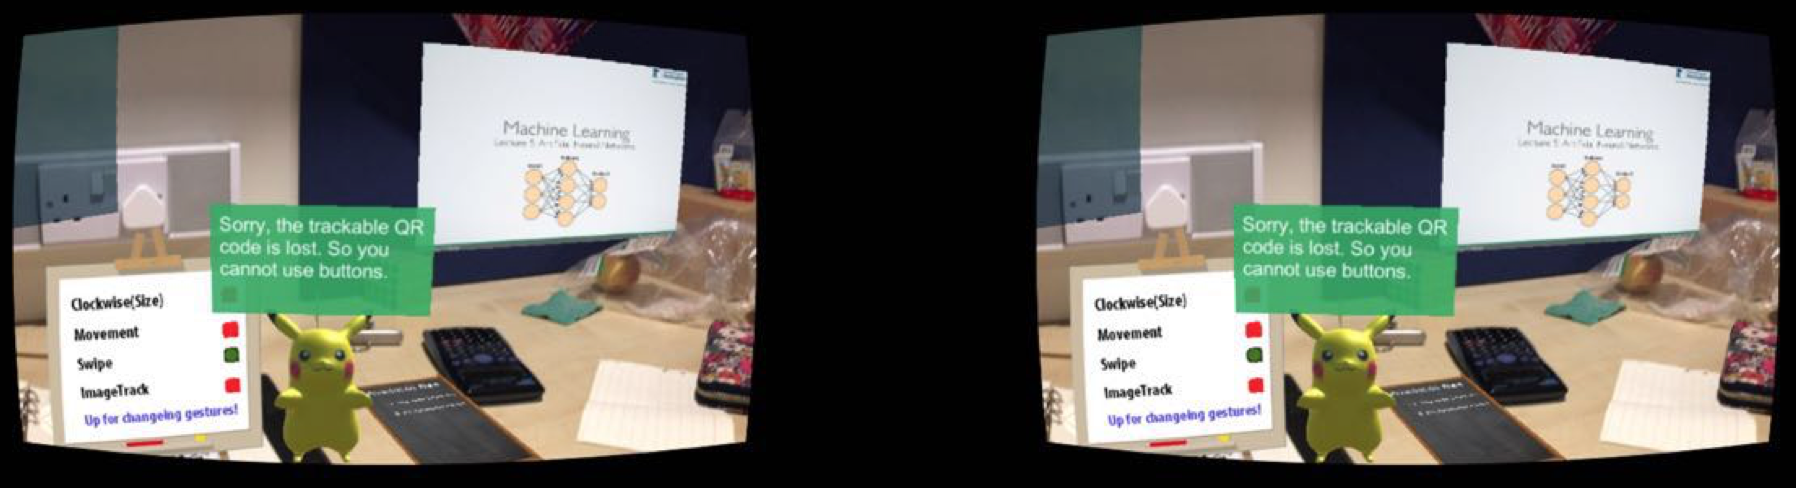
\includegraphics[width=\textwidth]{pdfreader}
    \caption{Implementation of PDF reader}
    \label{fig:mesh1}
\end{figure}
\\
Document lists will contain all the available materials, and it is displayed in a canvas as well. There is an if statement to check which PDF is displaying, and then update the string. For example, the use is viewing “G53MLE”, when the program finds this course in the documents arrayList, it will convert the string “G53MLE” to “-> G53MLE”. And from the user aspect, arrow point tells them title of PDF/PPT which is displaying.



\section{Hybrid desktop website}
In order to get access to this website(url), the user can not only type the URL in the web browser but also scan the initial QR code. Hybrid desktop website is used as the admin of this application. It provides a chance for the user to alter the database and get some basic information of this application. It is built with simple HTML, PHP and AngularJS. Besides, the website has a python Django server whose port is 8080 for making a python crawler to grab the weather information. It has four main sections: Introduction, task manager, online annotation and further.
\\
\\
Introduction and further section contains some simple HTML paragraphs and it is only used for showing new user a sketch of Hybrid Desktop and some potential implementation. Task Manager is the control board of tasks, all the tasks is displayed like a sticky notes. And at the top of the website, the user can typing their new task and behind the screen, some javascript will be used to check whether the user has actually typed something and if the user select “Please select your category”, the user will be able to enter his/her new category, but if he/she selects something, the input box will hide. 
\\
\\
These are coded with AngularJS’s SCOPE. The advantage of using AngularJS is it will not reload the page which can speed up the processing time and improve the user experience. So when the user click the delete or finish of the sticky notes, the AngularJs code will send an HTTP request to execute the MYSQL sentence and send the latest tasks back as an JSON array. Then the AngularJS code will assign these data to the SCOPE[17] which is an object that refers to the model of the application. It plays as the role of bridge between the view and the application controller which guarantee they are linked and update the value simultaneously.
\\
\\
Another important section is Annotation, it is used to link the “keyboard” with the “Hybrid Desktop”. Based on the previous survey that people prefer real keyboard, Annotation part is to create a platform for user to type in what they want and display that in the virtual annotation box. That page will have a 3 seconds interval to send a HTTP request to update the MYSQL database which enable that the virtual annotation box can retrieve the latest data. 
\\
\\
Below that typing section is an existing notes showing section. By selecting the category, the AngularJS code will request the PHP backend to retrieve the notes which belonged to the specific category and sent these notes back as a JSON array. By using ng-repeat, the user can see the selected notes without refreshing the pages. And the status button is used for helping the user to decide whether to display that note in the virtual world.
\\
\begin{figure}[h]
    \centering
    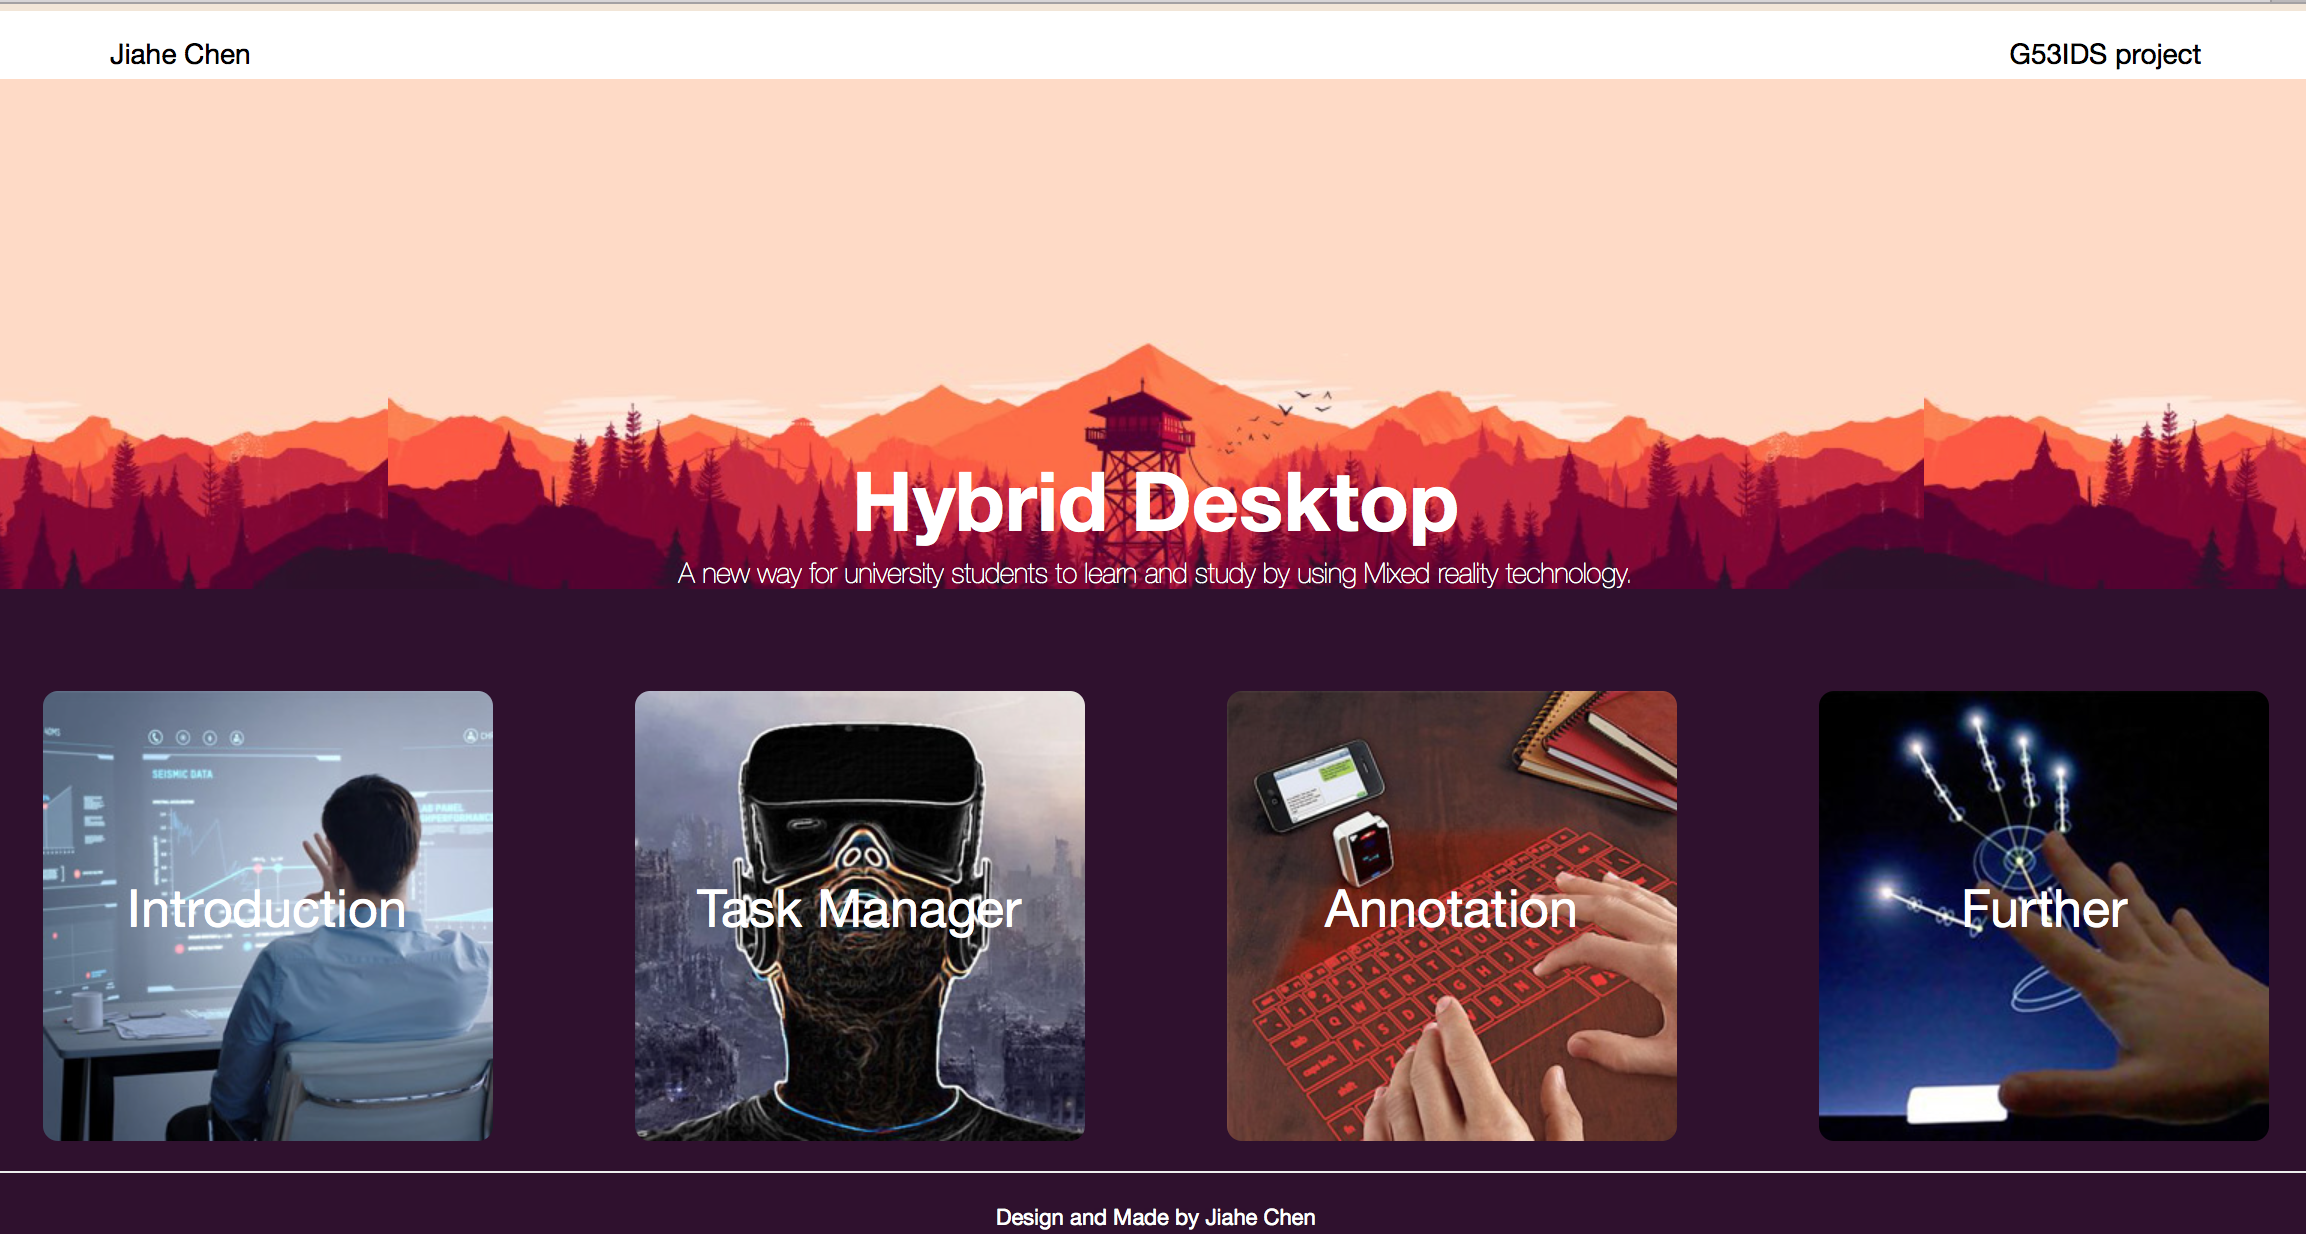
\includegraphics[width=\textwidth]{website}
    \caption{Hybrid desktop website main page}
    \label{fig:mesh1}
\end{figure}

\section{Bulletin board}
This project uses Unity’s Canvas to build the Bulletin board. Bulletin board has a HTTP GET to retrieve the existing tasks in the MYSQL database. The Bulletin Board is only used for displaying. Besides the displaying of tasks, the Bulletin board also shows some information about the weather and date. The weather is based on a python crawler to grab the data from BBC weather. The application will also get this weather information by a HTTP GET request. 
\\
\\
In order to get the latest tasks and weather information, it will call the HTTP GET request every 5 seconds which ensure that the display of tasks keeps synchronous with the databases and BBC weather. That means when the user add new tasks or the weather, the Bulletin board will refresh automatically. Also, the URL of Hybrid Desktop should be display as a string on it, and it will be more convenient for users to get access to it. The following figures show two implementations: one is the task manager page in Hybrid Desktop, and another is the bulletin board display. 
\begin{figure}[h]
    \centering
    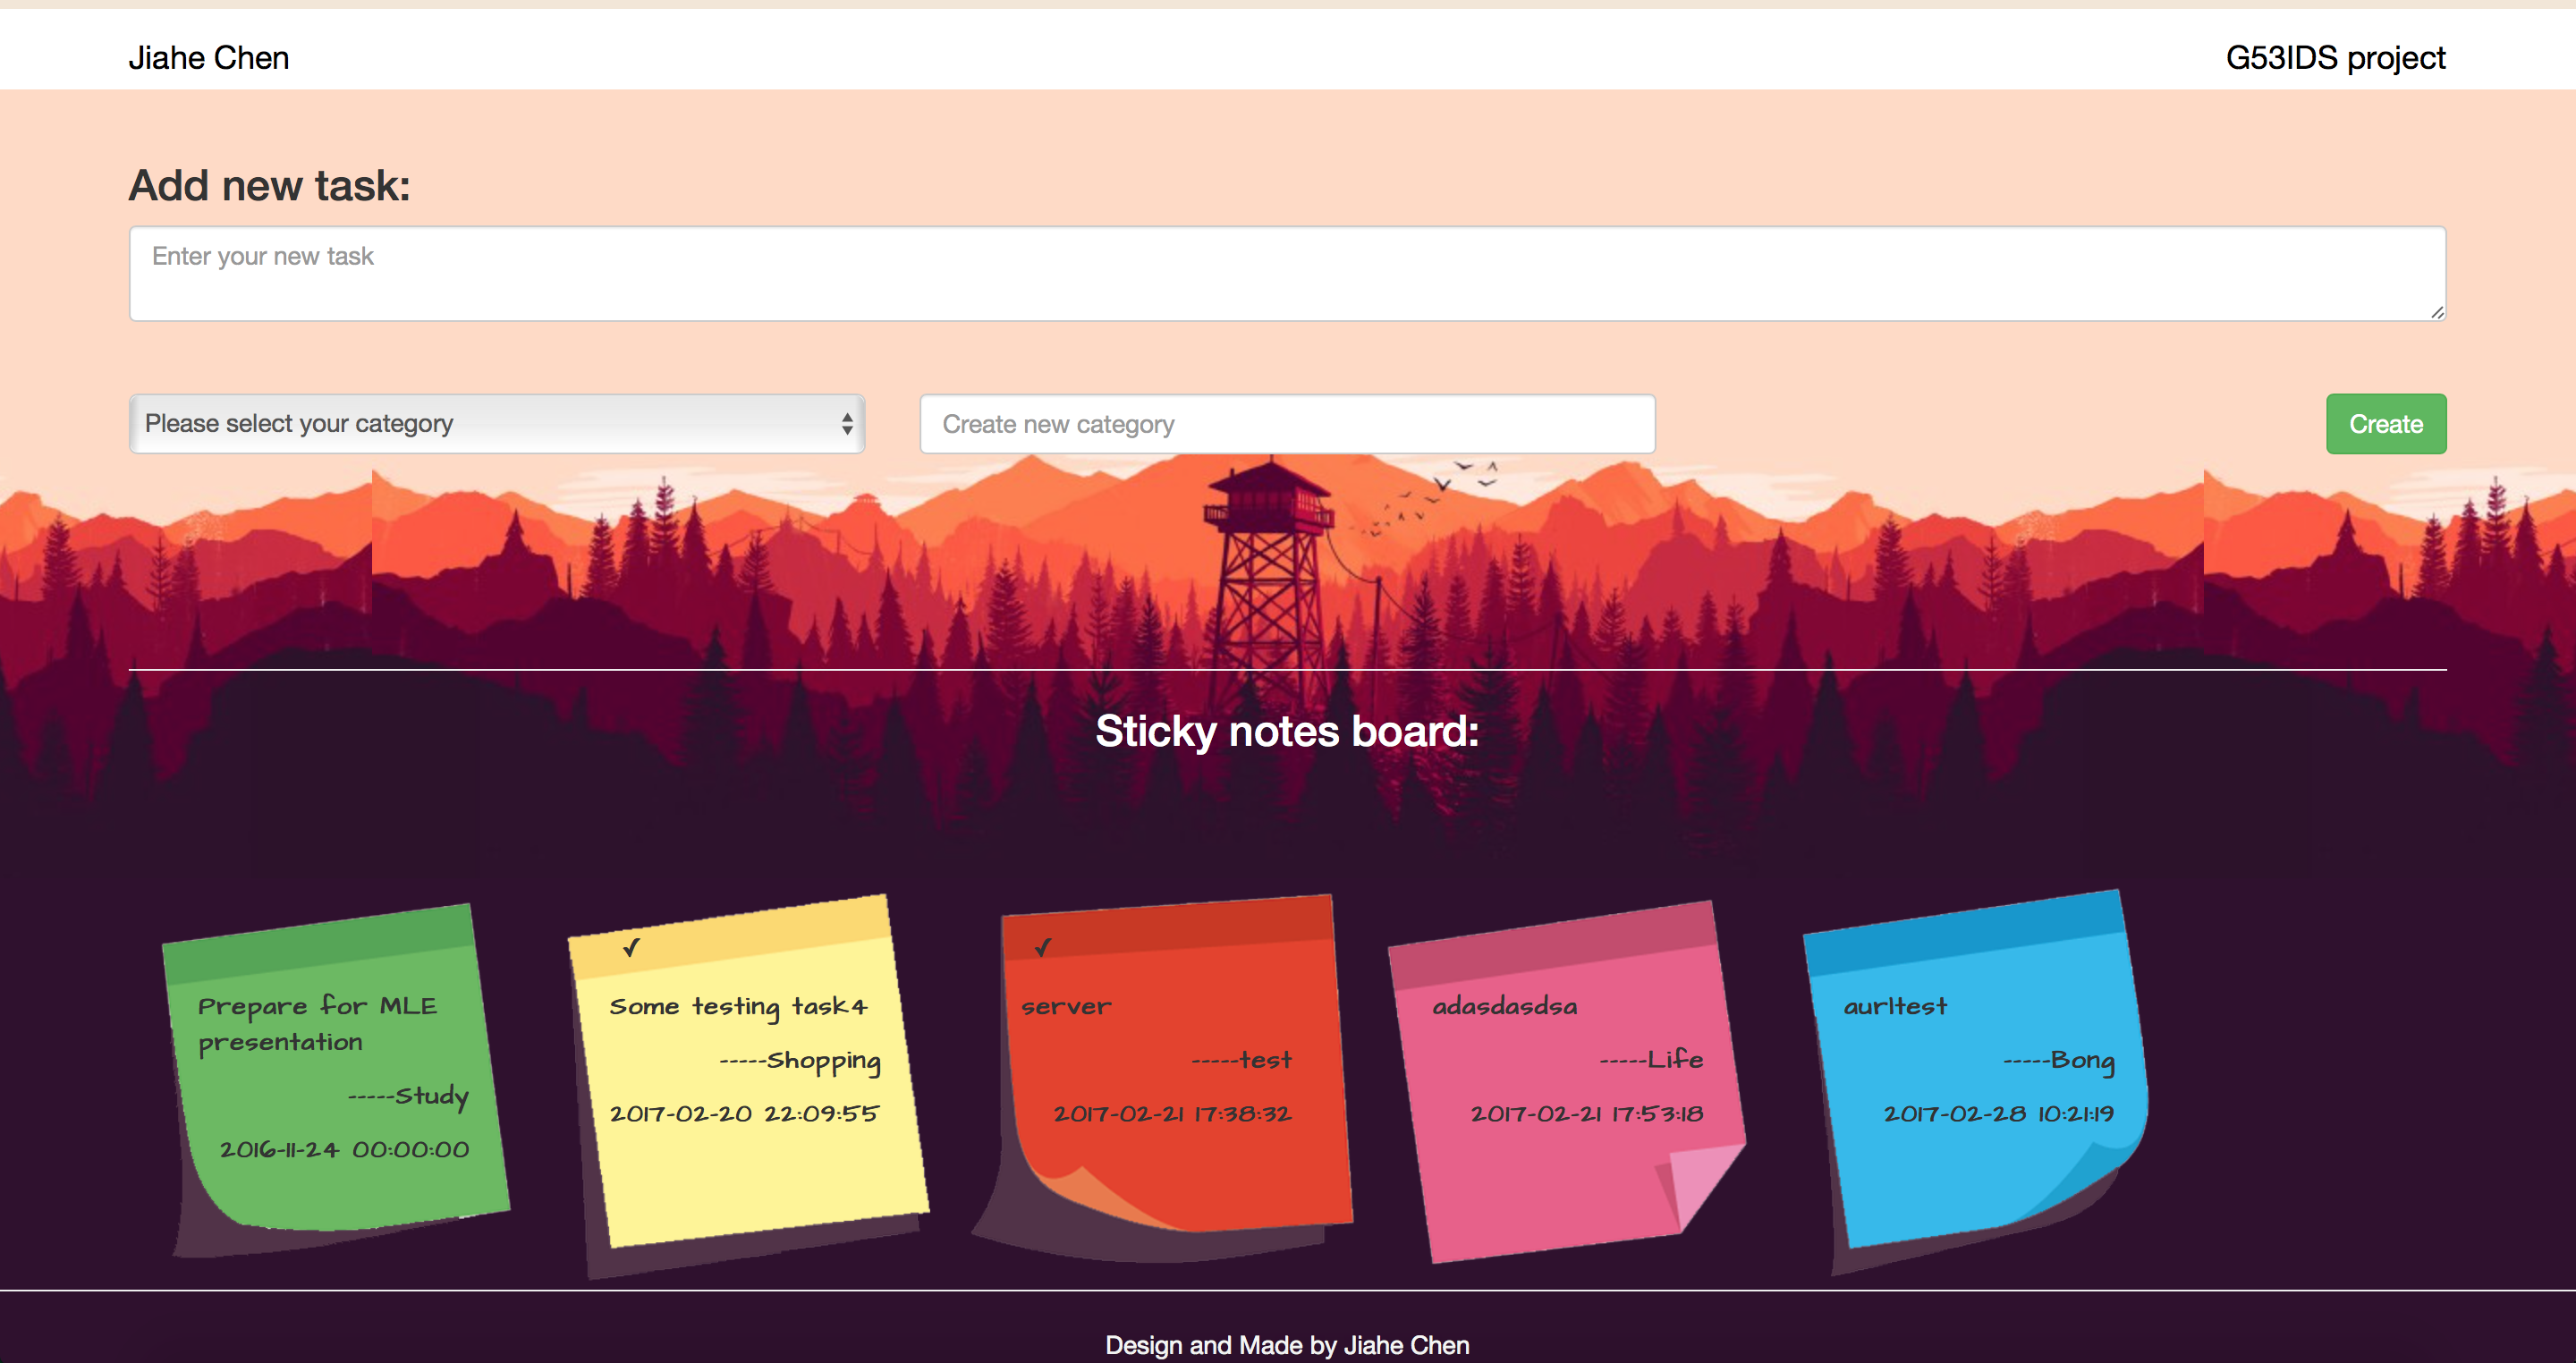
\includegraphics[width=\textwidth]{task}
    \caption{Hybrid desktop website task manager page}
    \label{fig:mesh1}
\end{figure}
\begin{figure}[h]
    \centering
    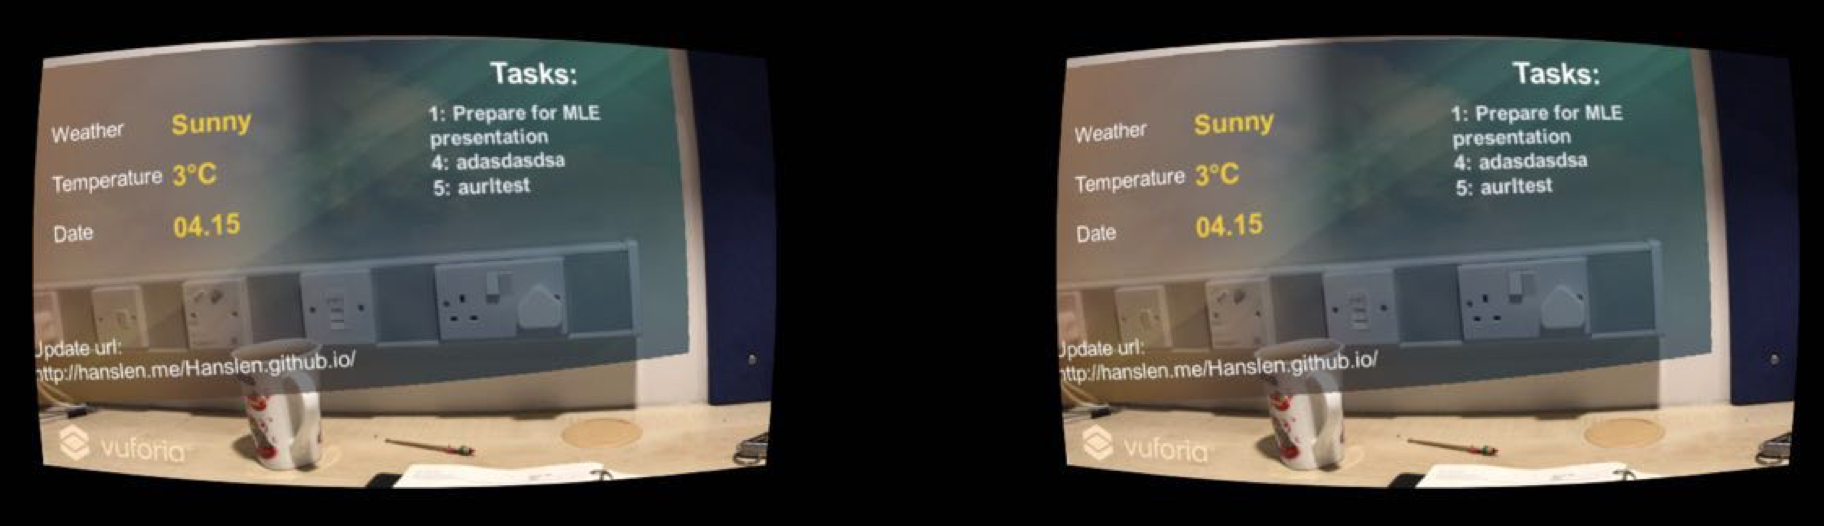
\includegraphics[width=\textwidth]{bulletin}
    \caption{Implementation of Bulletin Board}
    \label{fig:mesh1}
\end{figure}

\section{Electronic annotation displaying system}
The biggest problem of tracking these electronic annotations is where should they display. Because it should display in the correct position of the specific physical documents. There are two possible solutions: 1. Get the position of the annotation and store it in the database, when the user selects that annotation and wants to display that annotation, it requests a HTTP response and analyzes the position to help annotation display in the correct saved position. But the problem will cause by this implementation is the position is relevant to the position of camera. But each time, the physical documents may not be in the same place, and that can cause the annotation not showing above the physical document but in the wrong position. 
\\
\\
Another solution is inspired by imageTarget. It is possible to create another imageTarget and assign the annotation box be a child of that imageTarget. So when the camera recognizes the imageTarget, the annotation box can be moved by the changing position of imageTarget. Inside the annotation box it has a script which is used for updating what the user has typed. In the Hybrid Desktop website section, the methodology of online Annotation has been explained. And those AngularJs code ensures that the database contains the latest notes which the user is typing. And inside the annotation script, a WWW object of C\# will get the JSON object which contains the online annotation data and assign it to the title and annotation GAMEOBJECT’s text component’s text value. This implementation helps the annotation box contains what the user is typing or wants to display and it can be moved by the imageTarget.
\begin{figure}[h]
    \centering
    
\includegraphics[width=\textwidth]{annotation}
    \caption{Hybrid desktop website online annotation page}
    \label{fig:mesh1}
\end{figure}

\section{Leap Motion with iPhone}

Unlike Oculus which can use the Leap Motion API and Unity package directly. The current API of Leap Motion does not enable the developer to transfer data between Leap Motion and iPhone, but Leap Motion can be connect with Laptop and receive hand information. In order to control iPhone by using Leap Motion, socket communication could be used to transfer data. So in this section, some codes and methodology will be explained for how to make full connection with Leap Motion and iPhone. 

\subsection{Socket communication for server(PC) and client(iPhone)}
The System.Net.Sockets namespace contains some available socket interface and provides a chance for connecting Laptop with iPhone. In this Socket class, synchronous mode will be used because what the iPhone application(Client) needs is to perform receiving data wait until the Laptop(Server) gets data, transfers them to an identifiable command and sends it to the client. Synchronous socket enables this server application is suspended until it connects with a client. [15] In a similar way, when the client is connected with the server, it will be suspended until the server return a response which contains a command.[16] Because the application does not split into multiple independent tasks and servers, and it only has one thread for handling data. It is clear that synchronous socket is much more suitable than asynchronous socket.
\\
The basic principle of this implementation is like the following figure:
\\
\begin{figure}[h]
    \centering
	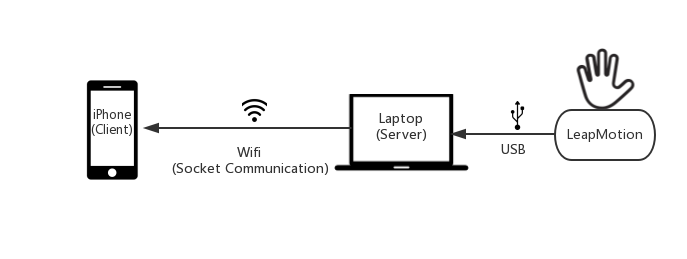
\includegraphics[width=\textwidth]{LeapMotionServer}
    \caption{Leap Motion with iPhone data transfer model}
    \label{fig:mesh1}
\end{figure}


\subsection{Coordinate system and Motion tracking data}
The coordinate system that used by Leap Motion system is right-handed Cartesian. In this project, users will need to put Leap Motion on the desktop rather than attached on the VR headset. In the virtual reality world, attached Leap Motion on the VR headset is preferable, and the reason is by analyzing these hand information, users are able to bring their bare hands in to virtual world, and what they can see and interact with is their virtual hands which is displaying by capturing their real hands and convert it to digital objects. But different from VR, this project is developed with AR technology which means users are seeing their real hands and interacting with their real hands. So because of different reference system, the position of hands will be a bit different in the virtual world and the real world. The information Laptop can received from Leap Motion is Frame Class which contains a list of tracked entities, and the entities this project are using are hands, fingers and gestures. 

\subsection{Conversion between gesture and command}
From Leap Motion API, the data program can get is the position of hand and it can also recognize some simple gestures. In this program, two gestures which are clockwise and counterclockwise are selected. As proposed functionality, these PDF reader should be able to zoom in and zoom out. Clockwise is the one of the natural and convenient behavior of people to do this command. So when the Leap Motion recognizes the circle gesture, the server will send a STRING to the client which is “clockwise” or “counterclockwise”. 
\\
\\
For the swiping gesture, it is developed based on the position of the hands. When the Leap Motion recognizes that there is a hand over the device, it will start to insert its position X in a FLOAT array whose length is 10. When it gets to the array[9], it will start to update the first element(array[0]) of the array. By doing these, it can ensure that this continuous array stands for the changing postitionX of hand. This array is the basic component to analyze which gesture the user is doing. If it is a continuous increasing array, the program will consider it as a swipe to next PDF gesture and send a STRING “next” to the client. If it is a continuous decreasing array, the program will consider it as a swipe to previous PDF gesture and send a STRING “previous” to the client. 
\\
\\
The problem will cause by only recognizing the positionX is when the user is doing a clockwise or counterclockwise gestures, it will have some probability that the array is continuous increasing or continuous decreasing. In order to avoid this wrong recognition, the application will have an enable and disable status for each gesture. For example, in the initial state, the enabling gesture is swiping and disabling gesture is circle and movement. If the user wants to change these status, he/she needs to hover his/her hand over the Leap Motion approximately 20cm (The reason for selecting this number is user performs their gesture almost between 0cm to 20cm, so when the hand is over 20cm, it can be considered as an uncommon position) for 3 seconds. When the program find that the position Y is over the defined constant, it will change the status (disable swipe and enable circle). From the user aspect, the status of these gestures will be presented in the instruction board as a virtual way. And the movement of the PDF reader is followed by the following principles:
\begin{figure}[h]
    \centering
	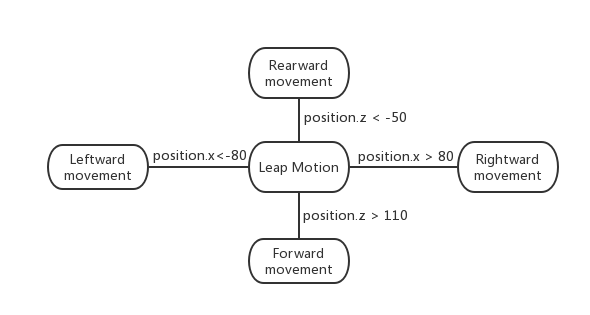
\includegraphics[width=\textwidth]{dtpos}
    \caption{PDF reader movement principles}
    \label{fig:mesh1}
\end{figure}



\subsection{Performing Leap Motion controlling with iPhone}
In the communication between Leap Motion and iPhone section, the iPhone can be considered as the client. And the data is received is not the position of hand but analyzed gesture of the user. This preprocessed conversion made the iPhone part more simple. It only need a switch case for implement different functions. And for future developers, they can send their gestures to the client and add more cases for performing their function. Because the client needs to be configured as the same IP as the server, and the WIFI port should not be blocked. In some WIFI environment, the C\# socket communication will not work due to the problem of port prevention.

\section{AI servant}
The display of the AI servant is based on the imageTarget, and the message box of AI servant will be updated based on the two components. The track of imageTarget and the Leap Motion potential gestures. Looking back to the Vuforia script, the project overwrites the 'DefaultTrackableEventHandler'. When the camera loses the track of the imageTarget, the message box will be updated to tell the user that it loses the track of the imageTarget. So, it will help the user has a clear view of the status of the digital objects. 
\\
\\
Another useful implementation is the Leap Motion potential gestures. It will tell the user what possible gesture it is performing, so each time, when the Leap Motion Client receives a data from the Leap Motion, it will update the AI servant message box. Based on the user feedback, they report that it is hard to track the changing status of the Leap Motion. In order to improve the user experience, the AI servant will also be used to tell the user the status of their progress. For example, when the user wants to disable some gestures and enable others, they will hover their hands over the leap motion for some seconds. In the origin version, they will not know whether the height which the Leap Motion has recognized is available and it is registering this gesture or not. In this version, it will show the progress which is indicated by a percentage number. When the loading progress is 100\%, it will start to enable and disable gestures. This is a clear view of the progress status.

